\section{Results III: Transferability and Generalization}
\label{sec:results_transfer}

This section reports the third block of the study: a pre-registered
transferability characterization of the hybrid recipe across three related
\boptest{} testcases that share the single-zone heating regime with
\texttt{bestest\_air} but differ structurally in actuator type, heat source,
or envelope scale. Unlike Sections~\ref{sec:results_fidelity} and
\ref{sec:results_control}, which both operate inside \texttt{bestest\_air},
this section asks the orthogonal question: \emph{which components of the
recipe transfer to a different testcase, and which do not?}

The pre-registration manifest
(\texttt{configs/block3\_testcase\_manifest.yaml}) was committed before any
non-\texttt{bestest\_air} \boptest{} run and is the third audit anchor in the
project (see Section~\ref{sec:experimental_setup}, paragraph on
reproducibility). All cell results below were appended to the manifest as
\texttt{cell\_results} entries without modification of the pre-registration
body; the manifest's commit history is therefore a verifiable timeline of
predictions logged before runs and results appended after runs.

\subsection{Pre-registered transferability protocol}
\label{ssec:res3_protocol}

The protocol crosses three testcases with three recalibration regimes and
applies a single quantitative verdict criterion per cell.

\paragraph{Testcase candidates.}
Three \boptest{} testcases were selected against four pre-registered
criteria: (a)~single-zone envelope, (b)~heating-capable HVAC, (c)~actuator
interface compatible with direct-supply-temperature command or overridable
through a documented adapter, and (d)~at least one structural difference
from \texttt{bestest\_air}. The chosen candidates are
\texttt{bestest\_hydronic\_heat\_pump} (primary; same envelope class,
hydronic loop with a heat pump replacing the air supply unit),
\texttt{bestest\_hydronic} (secondary; hydronic distribution with a boiler
and radiators), and \texttt{singlezone\_commercial\_hydronic} (stretch;
substantially larger envelope volume, hydronic distribution). Multi-zone
testcases and toy \boptest{} testcases were explicitly excluded.

\paragraph{Recalibration regimes.}
Each cell is run under one of three depths of recalibration:

\begin{itemize}
    \item \texttt{none}~--- the frozen \texttt{hybrid\_l010} thermostatic
    controller is deployed directly on the target testcase through an
    actuator adapter. No surrogate or controller is re-trained.
    \item \texttt{partial}~--- Stage~C residual head calibration is re-run
    on a prepared 15-minute target-testcase corpus. \czon{} is held frozen
    at the \texttt{bestest\_air} canonical value
    (\SI{4.413e5}{\joule\per\kelvin}); Stage~B is skipped. The controller
    remains frozen.
    \item \texttt{full}~--- the complete Stage~A/B/C pipeline is re-run on
    the target testcase. Stage~B re-identifies \czon{} from a new
    excitation-window subselection. The controller remains frozen.
\end{itemize}
Controller fine-tuning on the target-recalibrated surrogate is
\emph{explicitly excluded} from Block~3 per the manifest's
\texttt{scope.deliberately\_NOT\_claimed} list; that step belongs to a
separate follow-up study (see Section~\ref{sec:discussion}).

\paragraph{Verdict criterion.}
For each cell, the pre-registered verdict is
\(m_{s,\mathrm{RL}} \leq 1.25 \times m_{s,\mathrm{PI}}\) on the
testcase-specific yearly evaluation. Each testcase contributes its own
\boptest{} built-in PI yearly run as the normaliser. The \(1.25\times\)
slack accepts up to a $25\%$ degradation in composite KPI relative to the
default PI of that testcase; tighter post-hoc thresholds are permitted (the
slack can only be reduced, never widened, without violating
pre-registration).

\paragraph{Hypotheses.}
Four falsifiable hypotheses were logged before runs (manifest
\texttt{pre\_registered\_hypotheses} block):

\begin{itemize}
    \item \textbf{H1\textsubscript{strong}} (a priori $30\%$): frozen recipe
    deploys (regime~$=$~\texttt{none}) on $\geq 2$ of 3 testcases.
    \item \textbf{H2\textsubscript{medium}} (a priori $65\%$): partial
    recalibration brings $3/3$ to PASS on the thermostatic family.
    \item \textbf{H3\textsubscript{weak}} (a priori $85\%$): full
    recalibration brings $3/3$ to PASS on the thermostatic family.
    \item \textbf{Hierarchy consistency}: verdicts cannot worsen with
    deeper recalibration.
\end{itemize}

\subsection{Actuator interface and adapter}
\label{ssec:res3_adapter}

\texttt{bestest\_air} exposes a direct supply-temperature override, which
matches the thermostatic policy's action space. The three hydronic
testcases instead expose
\(\{\texttt{oveTSet\_u},\, \texttt{oveHeaPumY\_u},\, \texttt{ovePum\_u},\,
\texttt{oveFan\_u}\}\) (heat-pump variant) or the boiler/radiator analogue.
Block~3 transfer is therefore explicitly \emph{adapter-mediated}, not
literal direct-supply-temperature transfer. The adapter maps the frozen
policy's temperature-like action to a zone setpoint plus discrete on/off
overrides for heat pump, pump, and fan. The adapter is purely mechanical:
it does not learn or interpolate, and is identical across the three
testcases (substitutions are limited to which actuator IDs receive the
heating intent). Smoke tests confirmed that low and high override
combinations produce monotone changes in heat delivery on each testcase
before any controlled experiment was run.

\subsection{Per-testcase results}
\label{ssec:res3_per_testcase}

We report the three cells per testcase against the same pre-registered
criterion. Surrogate-side diagnostic measurements (predictive RMSE
improvement, \czon{} re-identification) are reported per cell as
\emph{diagnostic observations} alongside the controller verdict; they are
not controller verdicts in themselves.

\subsubsection{Primary testcase: \texttt{bestest\_hydronic\_heat\_pump}}

The frozen thermostatic policy routed through the hydronic adapter
produced yearly \(\msmetric = 0.665\) against
\(m_{s,\mathrm{PI}} = 0.464\); the \(1.25\times\) threshold was
\(0.579\). The cell therefore verdicts \textbf{FAIL} at
regime~$=$~\texttt{none}. Total annual heating energy was $7.3\%$ below PI;
the failure mode is comfort, not energy.

The partial regime (Stage~C heads only, with the
top-$5\%$-excitation subselection of the manifest) gave a useful
surrogate-side reduction at all rollout horizons: temperature RMSE moved
from \SI{0.977}{\celsius} to \SI{0.781}{\celsius} ($-20.1\%$) and power
mean-absolute error from \SI{2362}{\watt} to \SI{1768}{\watt} ($-25.1\%$).
\czon{} remained frozen at \SI{4.413e5}{\joule\per\kelvin} and the
Stage~B optimizer was not run, as required by the regime. Because the
controller was frozen and the adapter unchanged, however, the live yearly
\(\msmetric\) is identical to the \texttt{none} cell; the controller-side
verdict at \texttt{partial} is structurally \textbf{FAIL}.

The full regime re-identified \czon{} at
\SI{8.347e5}{\joule\per\kelvin} after $120$ Stage~B epochs, roughly
$1.89\times$ the \texttt{bestest\_air} canonical value. Temperature RMSE
dropped from \SI{1.421}{\celsius} to \SI{0.565}{\celsius} ($-60.2\%$) and
power MAE from \SI{2921}{\watt} to \SI{1767}{\watt} ($-39.5\%$). The
surrogate component therefore transfers successfully under full
recalibration. The controller-side verdict remains \textbf{FAIL} for the
same structural reason as \texttt{partial}.

\subsubsection{Secondary testcase: \texttt{bestest\_hydronic}}

The same protocol on the boiler-and-radiator testcase replicated the
pattern. The \texttt{none} cell produced \(\msmetric = 0.976\) against
\(m_{s,\mathrm{PI}} = 0.7502\) and a threshold of $0.9377$;
verdict \textbf{FAIL}. Annual energy was $5.84\%$ below PI; failure mode
was again comfort, not energy.

The full regime delivered the strongest surrogate-side numbers of the
three testcases: temperature RMSE moved from \SI{2.666}{\celsius} to
\SI{0.335}{\celsius} ($-87.4\%$) and power MAE from \SI{784}{\watt} to
\SI{85}{\watt} ($-89.2\%$). \czon{} was re-identified at
\SI{8.622e5}{\joule\per\kelvin}, i.e.\ $1.95\times$ the
\texttt{bestest\_air} value~--- within $3.2\%$ of the
\texttt{bestest\_hydronic\_heat\_pump} ratio. Controller verdict remained
\textbf{FAIL} by the same structural mechanism.

\subsubsection{Stretch testcase: \texttt{singlezone\_commercial\_hydronic}}

The larger commercial-scale testcase broke the binary FAIL pattern of the
two residential testcases but did so in a methodologically informative
way. The \texttt{none} cell produced \(\msmetric = 0.431\) against
\(m_{s,\mathrm{PI}} = 0.628\) and a threshold of $0.785$; the cell
\emph{satisfies the pre-registered threshold}, i.e.\ verdict
\textbf{THRESHOLD PASS}. However, annual energy was $35.3\%$
\emph{above} PI. The threshold PASS is therefore not a deployment PASS:
the composite \(\msmetric\) lies within tolerance because the building's
slower envelope dynamics absorb sustained overheating without breaching
the comfort band as severely as in the residential testcases, but the
energy penalty makes the operating point unfit for practical deployment.

The full regime re-identified \czon{} at \SI{8.429e5}{\joule\per\kelvin}
($1.91\times$ \texttt{bestest\_air}) and reduced temperature RMSE from
\SI{1.952}{\celsius} to \SI{0.238}{\celsius} ($-87.8\%$). The surrogate
component therefore transfers under full recalibration on the stretch
testcase as well.

\subsection{Aggregate findings on the N\,=\,3 hydronic family}
\label{ssec:res3_aggregate}

Two patterns emerge clearly across the three testcases.

\paragraph{Surrogate component is uniformly transferable.}
Full Stage~A/B/C recalibration produced $60.2\%$, $87.4\%$, and $87.8\%$
RMSE\textsubscript{T} improvements on the three testcases
(Figure~\ref{fig:component_decomp}a). \czon{} re-identification gave
ratios of $1.89\times$, $1.95\times$, and $1.91\times$ against the
\texttt{bestest\_air} canonical, with a spread of $3.2\%$
(Figure~\ref{fig:czon_consistency}).

\begin{figure}[t]
  \centering
  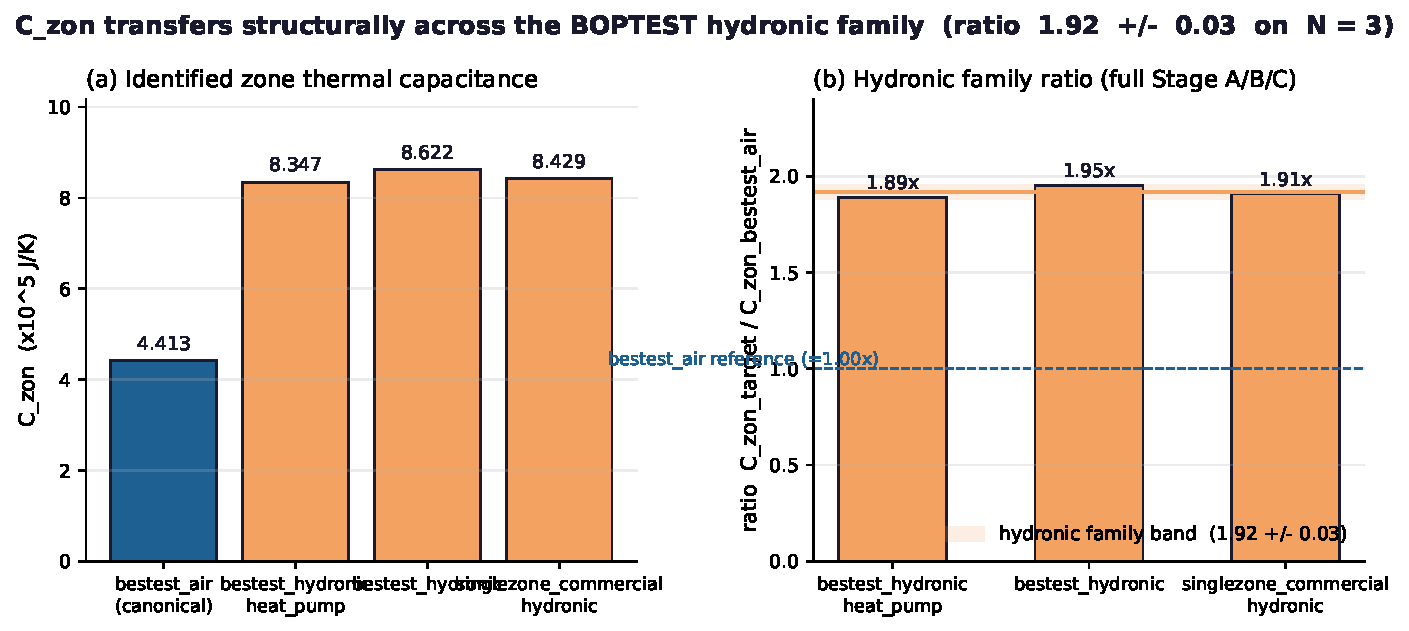
\includegraphics[width=0.95\linewidth]{figures/q1/C2_czon_consistency.pdf}
  \caption{Identified zone thermal capacitance $\czon$ across the
  \boptest{} hydronic family under full Stage~A/B/C recalibration.
  (a) Absolute $\czon$ values; (b) ratio relative to the
  \texttt{bestest\_air} canonical. The hydronic-family band
  ($1.91\pm0.03$) is the central numerical evidence for structural
  transferability of the surrogate component.}
  \label{fig:czon_consistency}
\end{figure}

\begin{figure}[t]
  \centering
  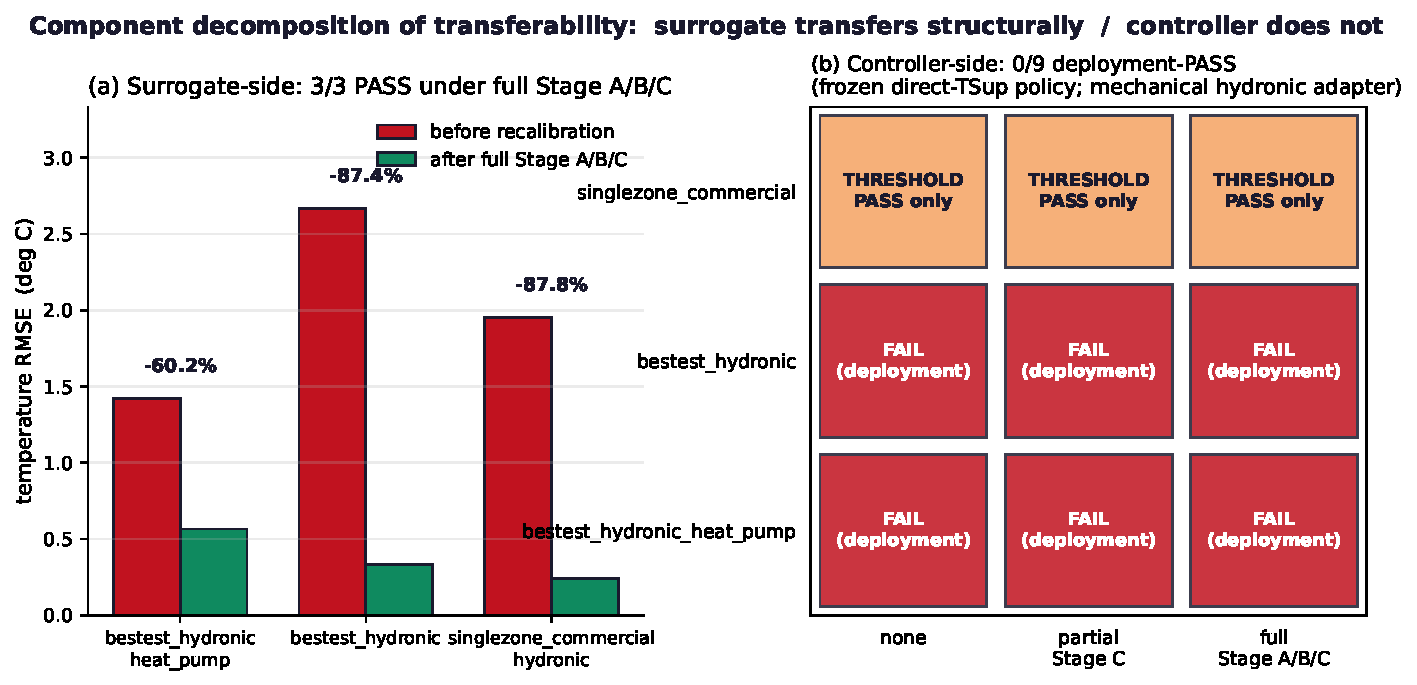
\includegraphics[width=0.95\linewidth]{figures/q1/C3_component_decomposition.pdf}
  \caption{Component-level decomposition of transferability across
  the \boptest{} hydronic family ($N=3$). (a) Surrogate-side
  temperature RMSE before and after full Stage~A/B/C recalibration:
  3/3 PASS, with $60$--$88\%$ RMSE reductions. (b) Controller-side
  verdict matrix: 0/9 deployment-PASS under the frozen
  direct-supply-temperature policy routed through a mechanical
  hydronic adapter. The asymmetry between the two panels is the
  central finding of Block~3.}
  \label{fig:component_decomp}
\end{figure} The Hou-and-Evins three-stage inverse calibration pipeline is
therefore demonstrably testcase-portable on the hydronic family. The
consistency of the \czon{} ratio --- in particular, its independence from
actuator type (heat pump vs.\ boiler) and from building scale (residential
vs.\ commercial) --- suggests that the hydronic family shares a
characteristic envelope thermal mass roughly $1.9\times$ that of
\texttt{bestest\_air} at the resolution of our inverse procedure.

\paragraph{Controller component is regime-dependent in its failure mode.}
Under the pre-registered frozen-controller scope, the controller fails on
all three testcases, but the failure manifests differently depending on
target dynamics:

\begin{itemize}
    \item On the two residential testcases
    (\texttt{bestest\_hydronic\_heat\_pump} and \texttt{bestest\_hydronic}),
    where envelope dynamics are fast relative to the controller's command
    horizon, failure manifests as a \emph{comfort-violation} mode:
    \(\msmetric\) is above the threshold because the policy's adapter-routed
    intent overshoots the comfort band.
    \item On the commercial testcase, where envelope dynamics are slower
    and the building absorbs heating overshoot without breaching the
    comfort band as severely, failure manifests as an
    \emph{energy-inflation} mode: \(\msmetric\) sits within the threshold
    but annual energy is $35.3\%$ above the PI reference.
\end{itemize}

Both failure modes reflect the same underlying mechanism: the controller
was trained on the direct-supply-temperature observation/action geometry
of \texttt{bestest\_air} and has no representation of the hydronic
actuator's intermediate variables (pump duty cycle, heat-pump on/off
gating, fan modulation). The adapter performs a mechanical mapping but
does not bring the policy's learned operating regime into alignment with
the target actuator's response curve. \emph{The transferability boundary
therefore lies in the controller-adapter interface, not in the surrogate
component.}

\subsection{Pre-registered hypothesis status at Block~3 closure}
\label{ssec:res3_hypotheses}

We resolve each pre-registered hypothesis explicitly:

\begin{itemize}
    \item \textbf{H1\textsubscript{strong}}: FALSIFIED. Frozen-recipe
    deployment at regime~$=$~\texttt{none} produced two clear FAIL
    verdicts and one threshold-PASS-with-large-energy-penalty; the strong
    claim that the recipe deploys without recalibration on $\geq 2$ of 3
    testcases in a deployment-ready sense is not supported.

    \item \textbf{H2\textsubscript{medium}}: FALSIFIED by structural
    definition. The partial regime keeps the controller frozen by
    pre-registered design, so the live KPI is identical to the
    \texttt{none} cell. Stage-C recalibration alone cannot rescue
    controller transferability without an accompanying controller-side
    update, which is scope-excluded.

    \item \textbf{H3\textsubscript{weak} (surrogate side)}: SUPPORTED on
    $N=3$. Full Stage~A/B/C recalibration consistently produces
    \(\geq 60\%\) RMSE\textsubscript{T} improvement and recovers a
    physically plausible \czon{} on every testcase.

    \item \textbf{H3\textsubscript{weak} (controller side)}: FALSIFIED with
    regime-dependent failure modes (as described above).

    \item \textbf{Hierarchy consistency}: SUPPORTED. No cell shows a
    verdict that improves at a shallower regime and worsens at a deeper
    one; surrogate fidelity is monotonically non-decreasing in
    recalibration depth.
\end{itemize}

The asymmetry between surrogate-side support and controller-side
falsification of the same nominal hypothesis (H3\textsubscript{weak}) is
precisely the central scientific content of Block~3: \emph{the recipe is
decomposable, and the two components transfer on different terms.}

\subsection{Threshold-framework limitation revealed by the commercial cell}
\label{ssec:res3_threshold_limitation}

The pre-registered verdict criterion was a single-axis threshold on the
composite \(\msmetric\). On the two residential testcases this criterion
worked cleanly: \(\msmetric\) exceeded threshold because comfort dominated
the composite weighting. On the commercial testcase the same criterion
returned PASS at a $35.3\%$ energy penalty, because the composite metric
trades comfort against energy and the PI baseline on that testcase was
already poor ($m_{s,\mathrm{PI}} = 0.628$, close to $1.0$).

We therefore distinguish two verdict levels post hoc, without weakening
pre-registration:

\begin{description}
    \item[Threshold PASS] \(m_{s,\mathrm{RL}} \leq 1.25 \times m_{s,\mathrm{PI}}\)
    (the pre-registered criterion).
    \item[Deployment PASS] Threshold PASS \emph{and} no individual KPI
    deteriorates by more than $25\%$ relative to PI in absolute terms.
\end{description}

The commercial testcase is Threshold PASS but not Deployment PASS at
regime~$=$~\texttt{none}, because the energy KPI deteriorates by $35.3\%$.
Reporting both levels gives a fairer picture of multi-objective trade-offs
in transferability studies than a single composite-threshold verdict
alone. This distinction is also flagged as a methodological observation
in Section~\ref{sec:discussion}.

\subsection{Scope-bounded claim and Block~4 follow-up}
\label{ssec:res3_scope_and_followup}

The defensible claim from Block~3, stated tightly, is:

\begin{quote}
On the \boptest{} hydronic family ($N=3$ testcases sharing single-zone
heating but differing in actuator, source, and envelope scale), the
Hou-and-Evins three-stage inverse calibration pipeline transfers the
surrogate component of our recipe with consistent physical-parameter
identification (\czon{} ratio $1.91 \pm 0.03$). The frozen
direct-supply-temperature controller, routed through a mechanical
hydronic adapter, does not transfer in a deployment-ready sense; its
failure manifests as comfort violation under fast envelope dynamics and
as energy inflation under slow envelope dynamics. The transferability
bottleneck is the controller-adapter interface, not the surrogate's
physics representation capacity.
\end{quote}

This finding closes Block~3 and identifies the natural follow-up: a
controller fine-tune step on the target-recalibrated surrogate, which the
present manifest pre-registers as out of scope. The Block~3
surrogate-side success establishes the prerequisite~--- that target
recalibrated surrogates are reliable enough to serve as fine-tune
environments~--- and the controller-side failure identifies the
bottleneck that such a fine-tune would have to close. We label this
direction \emph{Block~4} in the project's internal roadmap and treat it
as the most natural follow-up paper, deliberately deferred so as not to
expand the present manuscript beyond its pre-registered scope.

The \boptest{} commercial-scale result additionally raises a secondary
methodological point about how transferability is scored. The
threshold-versus-deployment distinction introduced in
Section~\ref{ssec:res3_threshold_limitation} is straightforwardly
generalisable: future transferability studies in HVAC reinforcement
learning would benefit from reporting tiered verdicts that combine a
composite-threshold pass with per-KPI absolute-degradation floors,
particularly when the PI reference itself is weak on the target
testcase.
